\documentclass[conference]{IEEEtran}
\IEEEoverridecommandlockouts
% The preceding line is only needed to identify funding in the first footnote. If that is unneeded, please comment it out.
\usepackage{cite}
\usepackage{amsmath,amssymb,amsfonts}
\usepackage{algorithmic}
\usepackage{graphicx}
\usepackage{textcomp}
\usepackage{xcolor}
\usepackage{array}
\usepackage[section]{placeins}
\usepackage{float}

\def\BibTeX{{\rm B\kern-.05em{\sc i\kern-.025em b}\kern-.08em
    T\kern-.1667em\lower.7ex\hbox{E}\kern-.125emX}}
\begin{document}

\begin{titlepage}
	\title{Cheap Autonomous Rovers for Multi-Agent Applications\\
		{\footnotesize \textsuperscript{*}Freedom Rover Units}
		\thanks{}}

	\author{\IEEEauthorblockN{1\textsuperscript{st} Jordy A. Larrea Rodriguez}
		\IEEEauthorblockA{\textit{Department of Electrical and Computer Engineering} \\
			\textit{University of Utah}\\
			Salt Lake City, USA \\
			Jordy.larrearodriguez@gmail.com}
		\and
		\IEEEauthorblockN{2\textsuperscript{nd}  Brittney L. Morales}
		\IEEEauthorblockA{\textit{Department of Electrical and Computer Engineering} \\
			\textit{University of Utah}\\
			Salt Lake City, USA \\
			brittneymrls@gmail.com}
		\and
		\IEEEauthorblockN{3\textsuperscript{rd} Misael Nava}
		\IEEEauthorblockA{\centerline{Department of Electrical and Computer Engineering} \\
			\textit{University of Utah}\\
			Salt Lake City, USA \\
			misaelnava812@gmail.com}
	}
	\maketitle
\end{titlepage}

\twocolumn

\begin{abstract}
The state of the art in autonomous swarms employs a decentralized model consisting of multi-agent networks. These robotic collaborative systems hold the potential to adapt to new environments and optimize individual performance to specific tasks without having to deal with global systems prone to single points of failure. Our team's focus lies therein in developing a multi-agent system capable of a decentralized network. The swarm will incorporates three two-wheel differential drive rovers interfaced through the Robot Operating System (ROS) via wifi telecommunication through the micro-ROS agent service. The central bay system consists of a single laptop to communicate objectives for the agents to complete (carefully designed demos). Our development stack will leverage ROS for project management, simulation capabilities, navigation libraries, and native server-client model in robotics applications. The rovers AI will incorporate simultaneous localization and mapping (SLAM) techniques for RT positioning based on a priori grid or map; thus, facilitating navigation through improved state space mapping. Thus, we introduce FRU-bot, an autonomous platform capable of deployment in decentralized and centralized systems.
\end{abstract}

\begin{IEEEkeywords}
Decentralized Communication, Swarm Communication, Multi-agent, ROS, Gazebo
\end{IEEEkeywords}

\section{Introduction}
\begin{figure}
	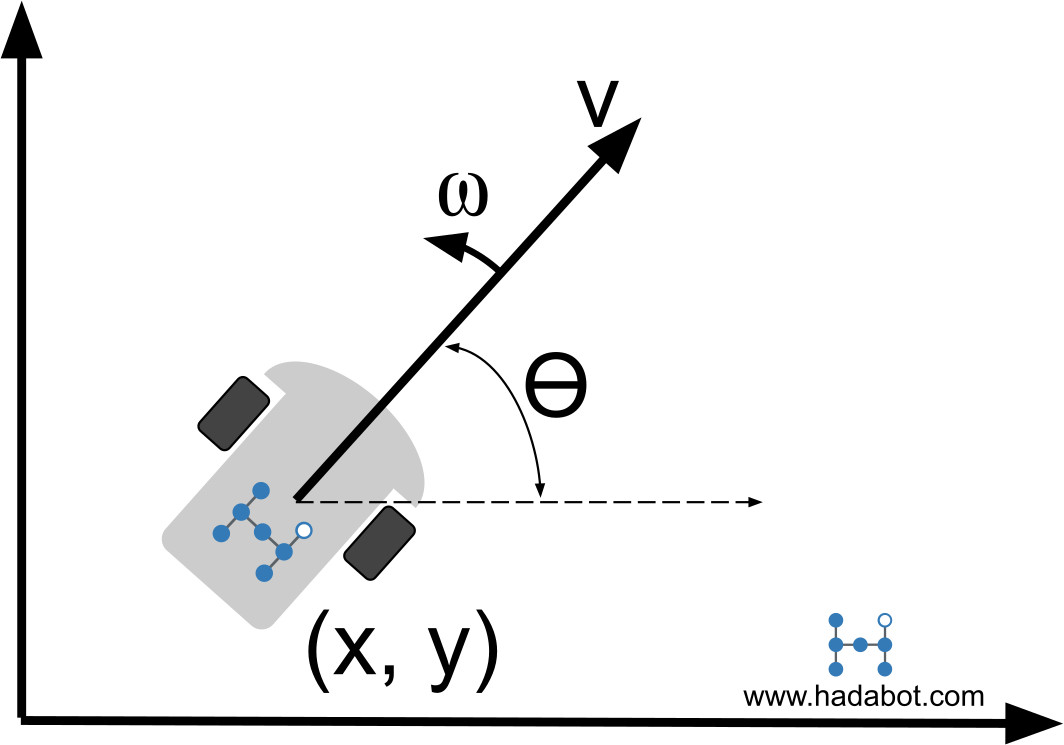
\includegraphics[width=\linewidth]{hadabot_unicycle_diagram_01.jpg}
	\caption{Graphical representation of 2D robot pose information standard to 2 wheel robots \cite{RN109}.}
\end{figure}
[Brittney]

\section{Background} 
A plethora of elements must come together to successfully deploy a swarm of decentralized agents. Our system requires a working knowledge in both the physical and abstract. The agents are subject to their physical characteristics: i.e., their circuitry, power consumption, mechanical components, sensors, processing power, and geometry to navigate and respond to an environment. The complexity that drives cyber-physical systems is what largely makes robotics difficult. An agent must be able to function perfectly in a world with a continuous state space. Today, researchers are seeing a high degree of success with robots that incorporate mathematical and data driven modeling that leverages the superior computational capabilities of modern processors to solve complex continuous problems in robotics. 
\subsection{Common Robot Autonomous Platforms} Common mobile platforms for autonomous robots encompass a range of designs tailored to diverse applications within the field of robotics. Wheeled platforms, such as differential drive and omnidirectional robots, are popular choices due to their simplicity and efficiency in navigating various environments. Differential drive platforms use two powered wheels, allowing the robot to turn and move forward or backward by adjusting the speeds of the wheels. Omnidirectional platforms, on the other hand, utilize special wheel configurations to achieve unrestricted movement in any direction. Lastly, tracked platforms offer enhanced traction and stability, making them suitable for challenging terrains.

One notable platform is the TurtleBot 3, a popular open-source robot platform widely used for research and education. TurtleBot 3, developed by ROBOTIS, is a compact and modular robot equipped with various sensors, including a 360-degree lidar sensor, a camera, and inertial measurement units (IMUs). Its differential drive system allows for omnidirectional movement, making it versatile for navigation in dynamic environments. The TurtleBot 3 is often employed in the development and testing of autonomous navigation algorithms, mapping techniques, and obstacle avoidance strategies. Its affordability, ease of use, and vibrant community support make it an attractive choice for researchers, students, and hobbyists interested in exploring the intricacies of autonomous robotics.

\subsection{Robot Localization}
\begin{figure}
	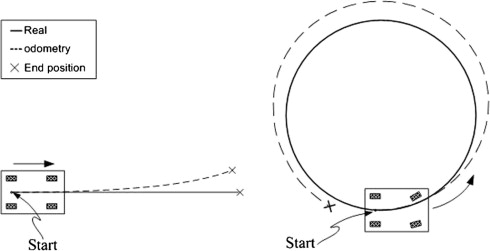
\includegraphics[width=\linewidth]{odometry_error.jpg}
	\caption{Graphical representation of basic odometry error as a robot follows a reference trajectory \cite{RN206}.}
\end{figure}
Normally, robots use a wide range of sensors to inform themselves about the surrounding environment. Our agents, for example, rely on a 6 axis inertial measurement unit (IMU) and rotatory encoders to produce an \{$X$, $Y$, $\theta$, $\dot{X}$, $\dot{Y}$, $\dot{\theta}$, $\ddot{X}$, $\ddot{Y}$\} state configuration at every time step by considering physical properties and mechanics (Fig. 1). However, a frequent problem with using rudimentary techniques solely for odometry is that error propagated at each time step due to environmental conditions, sensor specifications, electrical noise, and rounding error can deviate a naive agent during localization. The problem persists even with the use of a known map and highly accurate sensors. Consider how a human might traverse a city by using a map. The human could ensure their own position by simply pondering their place in respect to features of the map like buildings, intersections, or street signs. Even if the human absent mindlessly navigated the city, they could triangulate their location by simply calculating their positions based on observations (such as the coffee shop across the street). Our robots, incorporate a Kalman ExFor an agent, SLAM leverages known knowledge of poses at past time steps and emissions or observations (sensor readings) made as the agent accumulates error through basic odometry to calculate probabilities of where the agent can be in space. Any number of sensors that detect 'emissions' from the environment can be used for SLAM; however, 2D lidar and cameras are regularly used for the high degree of precision awarded. Agents are capable of both learning a new environment and updating a known map with SLAM; thus, justifying our deployment of SLAM to improve the navigation capabilities of each agent.

\subsection{Robot Kinematics} <Jordy>

\subsection{ROS2 and Open Source Frameworks} <Jordy>

\subsection{Robot Description and Transformation Trees} <Jordy>

\subsection{Gazebo for Robot Simulation} <Jordy>

\subsection{Autonomous Navigation} <Jordy>

\subsection{Multi-Agent Swarm Systems} <Jordy>

\section{Project Implementation}
\subsection{Prelminary Robot Chassis}

\subsection{Preliminary Electronics Design and Testing}

\subsection{Preliminary ROS2 Robot Description Design and Simulation}

\subsection{Hardware/Firmware}

\subsection{Multi-Agent Implementation with ROS2}

\section{Evaluation}

\subsection{Conclusion}

\subsection{Appendices}

\section{Discoveries and Pitfalls}  

\nocite{*}
\bibliographystyle{ieeetran}
\bibliography{citations}% Produces the bibliography via BibTeX.
\vspace{12pt}

\end{document}